%\section*{Acknowledgment}
%This work was supported by the National Research Foundation of Korea (NRF) grant funded by the Korea government (MSIT) (No. RS-2025-24803208) and the Institute of Information \& Communications Technology Planning \& Evaluation (IITP) grant funded by the Korea government (MSIT) (No. RS-2020-II201336, Artificial Intelligence Graduate School Program (UNIST)). This work was supported by a New Faculty Research Grant of Pusan National University, 2025.

%\section*{CRediT authorship contribution statement}
%Youngbin Lee: Writing – original draft, Writing – review \& editing, Data curation, Formal analysis, Visualization, Software. Yejin Kim: Writing – original draft, Writing – review \& editing, Data curation, Formal analysis, Visualization, Software. Juhyeong Kim: Writing – original draft, Data curation, Discussion. Suin Kim: Writing – original draft, Discussion. Yoontae Hwang: Writing – review \& editing, Methodology, Funding acquisition. Yongjae Lee: Writing – original draft, Writing – review \& editing, Methodology, Visualization, Funding acquisition.

\section*{Declaration of generative AI and AI-assisted technologies in the manuscript preparation process}
During the preparation of this work the author(s) used Gemini 2.5 Pro in order to refine the grammar and tone of the written text. Importantly, the research results, including the development of the code and the core scientific contributions, were carried out entirely without the assistance of LLMs. After using this tool/service, the author(s) reviewed and edited the content as needed and take(s) full responsibility for the content of the published article.

\section{Prompt Design Details} \label{appendix:prompts}

To clarify the temporal context for the return prediction task, we include an explicit reference date in the system prompt. This date represents the point in time at which the LLM is expected to provide its analysis—positioned between the past time series data and the future return period. By anchoring the prediction task to a specific date, we help the model better interpret the directionality of the input data and generate temporally coherent forecasts.

To ensure consistent and parseable responses from the LLMs, we adopt a structured output format using the JSON schema supported by the chat completions API endpoint. This approach standardizes the outputs across all LLMs and ensures that each model provides consistently structured responses across repeated queries, reducing the likelihood of formatting errors and facilitating reliable downstream processing.

To enhance the models' numerical sensitivity, all daily return inputs are scaled by 100 (i.e., presented in percentage terms). For instance, a daily return of -0.0036 is provided as -0.36. This scaling prevents issues arising from the small magnitude of raw daily returns, which can be difficult for LLMs to differentiate and process effectively. This approach is analogous to using basis points in finance to handle small numerical values. By providing a rich, multi-faceted data context and clear instructions, the prompts enable the LLMs to generate informed, quantitative views for portfolio construction.

\begin{figure}[htbp]
\centering
    \scalebox{0.92}{%
    \begin{tcolorbox}[colframe=blue!80!black, colback=blue!10!white, coltitle=white, title=System Prompt, width=1.08\columnwidth]
    \scriptsize
    \setlength{\itemsep}{1pt}%
    \setlength{\topsep}{2pt}%
    \setlength{\partopsep}{0pt}%
    \setlength{\parsep}{0pt}%
    You are providing analysis on \texttt{{\{\{DATE\}\}}}. Predict the average daily return for the next two weeks based on the information provided about a stock's past performance.
    You will receive the following inputs:
    \begin{itemize}
        \item \textbf{Daily Returns}: The stock's daily returns, a time-series from the past two weeks.
        \item \textbf{Company Sector}: The company's GICS sector classification.
        \item \textbf{Sector Returns}: The company sector's daily returns, a time-series from the past two weeks.
        \item \textbf{Market Returns}: The S\&P 500's daily returns, a time-series from the past two weeks.
        \item \textbf{Company Information}:
            \begin{itemize}
                \item Ticker: The stock symbol.
                \item Company Name: The name of the company.
                \item GICS Sector: The Global Industry Classification Standard sector.
                \item GICS Sub-Industry: The sub-industry classification.
            \end{itemize}
    \end{itemize}
    
    \# Steps
    \begin{enumerate}
        \item \textbf{Analyze the Time-Series Data}: Review the historical daily returns to identify patterns, trends, or anomalies that may affect future performance.
        \item \textbf{Consider Sector Performance}: Analyze how the market and the sector's performance might influence the stock's future returns.
        \item \textbf{Incorporate Company Information}: Use the details from the GICS sector and sub-industry, along with the company symbol and name, to contextualize the predicted performance within its industry.
        \item \textbf{Predict Future Returns}: Estimate the average daily returns for the next two weeks based on the analysis of available data.
    \end{enumerate}
    
    \# Output Format
    \begin{quote}
    Return a single float value that represents the predicted average daily return for the stock over the next two weeks, without any additional commentary or explanation.
    \end{quote}
    
    \# Notes
    \begin{itemize}
        \item Ensure the prediction considers the quantified data from the time-series.
        \item Make calculations based on statistical trends from daily returns data.
        \item Pay attention to the trends within both the stock's daily returns and the market's return data.
        \item Consider the relevance of the company's sector to refine your predictions.
        \item Make calculations without additional interpretation or commentary.
    \end{itemize}
    
    \end{tcolorbox}%
    }
    \caption{The structure of the system prompt used to elicit return forecasts from the LLMs.}
    \label{fig:system_prompt}
\end{figure}



 % \label{fig:system_prompt}

\begin{figure}[htbp]
\centering
    \scalebox{0.92}{%
    \begin{tcolorbox}[colframe=green!60!black, colback=green!5!white, coltitle=white, title=User Prompt, width=1.08\columnwidth]
    \scriptsize
    \ttfamily % Use a typewriter font for code-like text
    \textbf{Daily Returns:} [-1.17, -0.92, -2.31, -0.36, -3.02, 2.53, 0.1, -0.23, 0.45]
    
    \vspace{0.5mm}
    \textbf{Company Sector:} Information Technology
    
    \vspace{0.5mm}
    \textbf{Sector Returns:} [-0.14, -0.38, -1.88, 0.03, -1.1, 2.38, -0.41, 0.17, -0.31]
    
    \vspace{0.5mm}
    \textbf{Market Returns:} [0.09, -0.39, -1.61, -0.04, -0.67, 2.05, -0.56, 0.4, -0.01]
    
    \vspace{0.5mm}
    \textbf{Company Information:}
    
    \hspace{5mm} \textbf{Ticker:} AAPL
    
    \hspace{5mm} \textbf{Company Name:} Apple Inc.
    
    \hspace{5mm} \textbf{GICS sector:} Information Technology
    
    \hspace{5mm}     \textbf{GICS sub-industry:} Technology Hardware, Storage \& Peripherals
    
    \end{tcolorbox}%
    }
    \caption{An example user prompt providing data for Apple Inc. (AAPL) on a specific rebalancing date.}
    \label{fig:user_prompt}
\end{figure} % \label{fig:user_prompt}

\section{Detailed Model-Level Statistics} \label{appendix:LLM}

\subsection{View Statistics}

Table~\ref{tab:view_statistics} provides the summary statistics for the entire population of raw views generated by each LLM throughout the test period. These statistics reveal the distinct predictive ``styles" of the models that were discussed in the main analysis. For instance, \textbf{\texttt{Llama}} is characterized by the highest mean return but also the largest standard deviation and the widest min-max range, indicating a high-conviction, high-dispersion approach. In contrast, \textbf{\texttt{Qwen}} shows the lowest standard deviation, reflecting a more cautious and stable view generation process, while \textbf{\texttt{Gemma}} is notable for its negative mean, confirming a persistent pessimistic bias. These underlying statistical properties are the root cause of the performance differences analyzed in the main text.

\begin{table}[h!]
    \centering
    \caption{Summary Statistics of LLM-Generated Views}
    \label{tab:view_statistics}
    \renewcommand{\arraystretch}{1.2}
    % siunitx 설정: 숫자를 소수점 4자리로 정렬
    \sisetup{
        round-mode=places,
        round-precision=4,
        table-format=-2.4 % 부호, 정수 2자리, 소수 4자리
    }
    \small
    \setlength{\tabcolsep}{5pt}
    \begin{tabular}{l S S S S}
    \toprule
    \textbf{Metric} & {\textbf{\texttt{Gemma-7B}}} & {\textbf{\texttt{Qwen-2-7B}}} & {\textbf{\texttt{Llama-3.1-8B}}} & {\textbf{\texttt{GPT-4o-mini}}} \\
    \midrule
    \textbf{Count}      & \multicolumn{1}{c}{1000} & \multicolumn{1}{c}{1000} & \multicolumn{1}{c}{1000} & \multicolumn{1}{c}{1000} \\
    \textbf{Mean}       & -0.3847       & 0.1007        & 0.1786        & 0.1347        \\
    \textbf{Std}        & 0.7492        & 0.2430        & 0.2248        & 0.4171        \\
    \textbf{Min}        & -2.5617       & -1.1486       & -0.5812       & -2.9331       \\
    \textbf{25\%}       & -0.9917       & 0.0159        & 0.0290        & -0.0299       \\
    \textbf{Median}     & -0.5152       & 0.0343        & 0.1169        & 0.1295        \\
    \textbf{75\%}       & 0.1607        & 0.1519        & 0.2923        & 0.3191        \\
    \textbf{Max}        & 2.6854        & 1.2284        & 1.1264        & 2.6172        \\
    \bottomrule
    \end{tabular}
\par\small\textit{Note:} All metrics except `Count' are expressed in percentages (\%).
\end{table} % \label{tab:view_statistics}

% \subsection{Analysis of Forecasting Errors} % 

% Table~\ref{tab:prediction_errors} presents an analysis of the forecasting accuracy for the views generated by each LLM and for the traditional estimate used by the MVO benchmark. The table quantifies the prediction error by comparing the expected returns—either generated by an LLM or, in the case of MVO, estimated from the historical average of past returns—against the actual realized returns of the subsequent period. This error is measured using three standard metrics where lower values are better: Mean Squared Error (MSE), Root Mean Squared Error (RMSE), and Mean Absolute Error (MAE).

% The results reveal a strong correspondence between a model's forecasting accuracy and its ultimate portfolio performance, as detailed in Table~\ref{tab:vertical_performance_comparison}. \textbf{\texttt{BLM-Qwen}} and \textbf{\texttt{BLM-Llama}}, which demonstrated the highest predictive accuracy by achieving the lowest errors across all three metrics, also generated the portfolios with the best absolute and risk-adjusted returns (CAGR and Sharpe Ratio respectively). This provides direct evidence that their outperformance was rooted in a superior underlying ability to forecast market returns. Conversely, the MVO benchmark, relying on naive historical averages, exhibited high prediction errors and correspondingly poor investment results. Interestingly, while \textbf{\texttt{BLM-Gemma}} also showed high forecasting errors—even worse than MVO's—its final portfolio outperformed both MVO and \textbf{\texttt{BLM-GPT}} in terms of CAGR. This suggests that within the Black-Litterman framework, the nature of the views can be as important as their raw accuracy; the consistent (though pessimistic) bias of Gemma may have provided a more stable, albeit flawed, signal for the optimizer to work with.

%\section{Analysis of Portfolio Allocation Dynamics}
%Figures~\ref{fig:weights_change_LLM} and~\ref{fig:weights_change_baselines} illustrate the temporal evolution of portfolio allocations for the LLM-driven and baseline strategies, respectively. Figure~\ref{fig:weights_change_LLM} details the asset weights at each rebalancing date for the portfolios constructed using our proposed framework. The allocations shown are dynamically adjusted based on the predictive views generated by each respective LLM. For comparison, Figure~\ref{fig:weights_change_baselines} displays the allocations for the baseline portfolios. These include the static, uniformly distributed EW strategy and the MVO portfolio, whose weights are derived solely from historical data. 

%\begin{figure*}[ht]
%    \centering
%    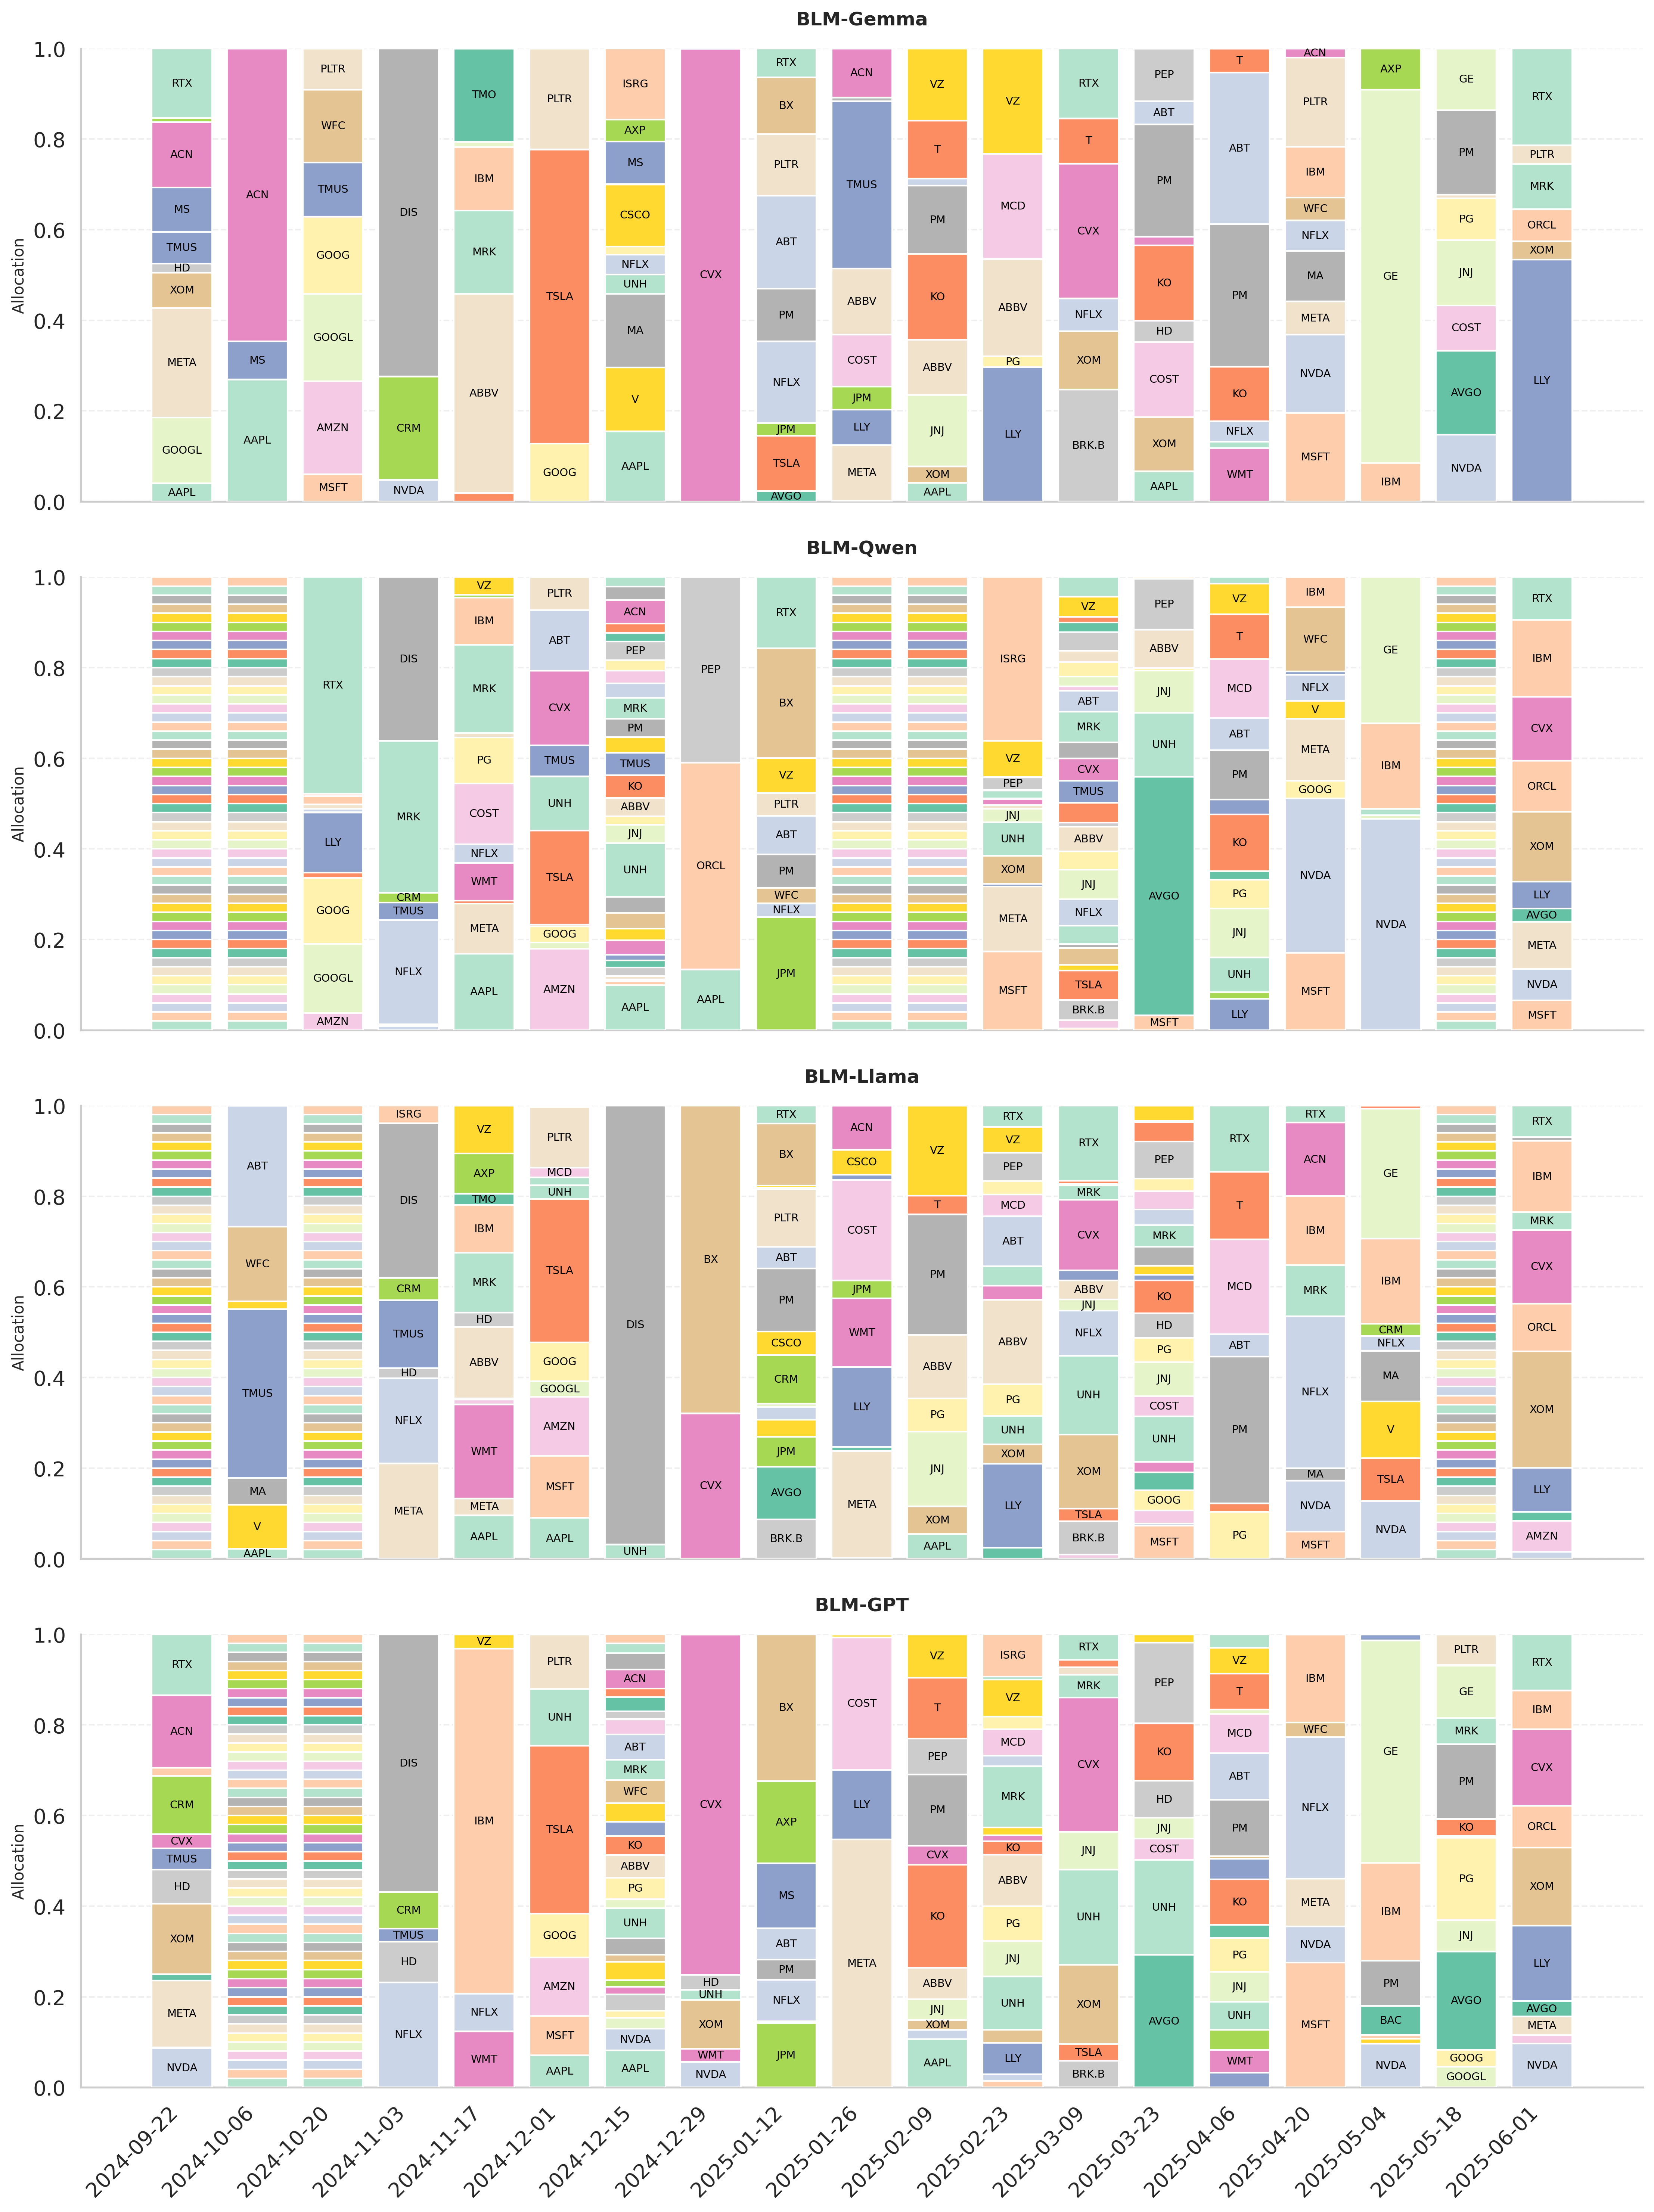
\includegraphics[width=1\linewidth, height=1\textheight, keepaspectratio]{figure/weights_change_LLM.png}
%    \caption{Time-series of Asset Allocation Weights for \textbf{BLM Portfolios}}
%    \label{fig:weights_change_LLM}
%\end{figure*}

%\begin{figure*}[ht]
%    \centering
%    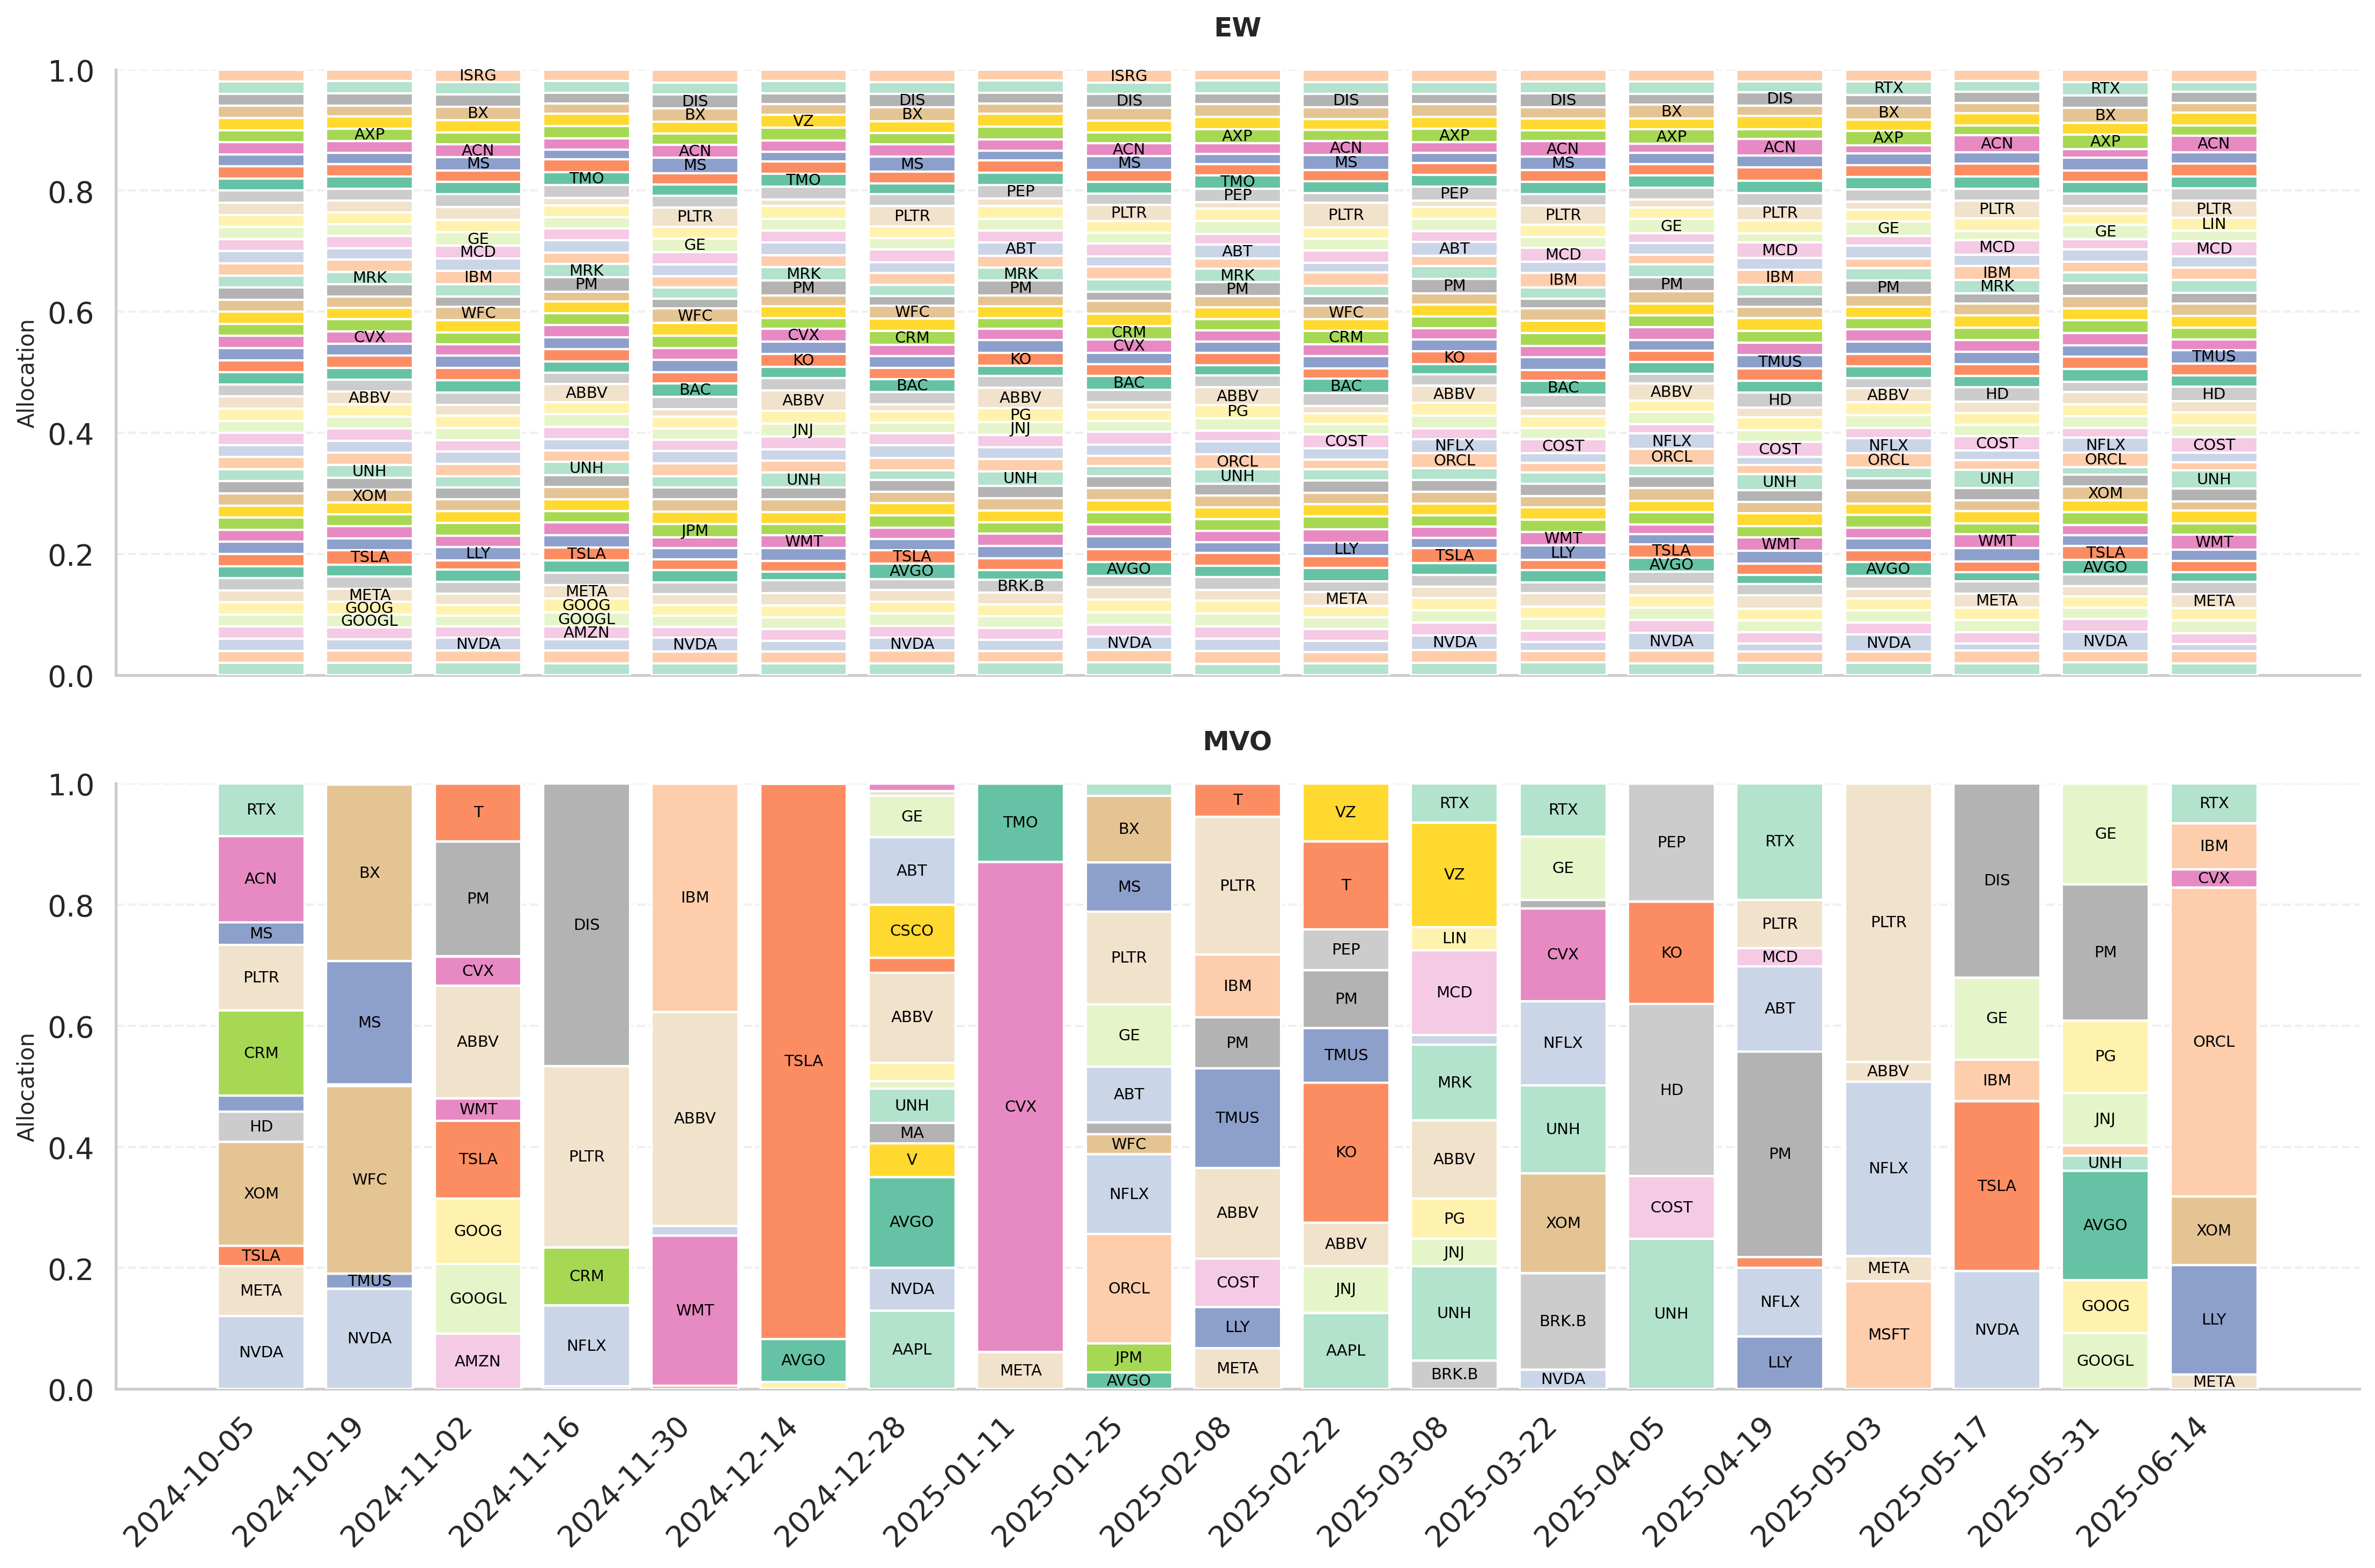
\includegraphics[width=1\linewidth, height=1\textheight, keepaspectratio]{figure/weights_change_baselines.png}
%    \caption{Time-series of Asset Allocation Weights for \textbf{Baseline Portfolios}}
%    \label{fig:weights_change_baselines}
%\end{figure*}